%\large\zihao{-4}
%-----------------------------------------
\begin{center}
	{\heiti\bf\LARGE\zihao{3}{\biaoti\\}}
%	{\bf\LARGE\zihao{3}{\enbiaoti\\}}
%	{\enbiaoti}
	
	\vspace{0.3cm}
	{\heiti\bf\LARGE\zihao{-4}\minzi}
	
	{\zihao{5}\university\school,\city}
	
	{\zihao{5}zhongshengyanzy@foxmail.com}
\end{center}

%------------------------------------

%\begin{center}
%\begin{minipage}[t]{7cm}
\noindent{\zihao{5}{\bf 摘要:}
	\fangsong
	% 请填入中文摘要:
	DDoS攻击是网络安全领域中的重要问题之一,而SDN技术的出现为DDoS攻击的检测和防御提供了新的思路和手段。本文利用mininet平台模拟SDN架构进行网络流量监测研究,通过SDN架构实时监控流量信息的变化,并对DDoS攻击做出及时处理,实现了高效的DDoS攻击检测和精准的攻击源定位,有效地提高了网络安全防御能力。
}\vspace{0.1cm}
%\end{minipage}
%\end{center}
%\end{multicols}
%\begin{multicols}{2} 
\begin{multicols}{2} 
\section{引言}\label{chpt:1}%===============================================
分布式拒绝服务攻击(DDoS)是一种通过同时向目标网络中发送大量伪造的流量,导致目标网络服务不可用的攻击方式。DDoS攻击对全球范围内的各种类型的网络造成了严重的威胁,从小型网络到政府和金融机构的大型数据中心都可能成为攻击目标。DDoS攻击的主要目的是使网络服务不再响应,从而导致网络的瘫痪。这种攻击对于企业和组织而言,可能会带来严重的经济损失和信誉问题。

目前,DDoS攻击的检测和防御成为网络安全领域的重点研究问题之一。然而,传统的检测和防御方法通常是基于网络流量的规律性和特征的预测和分析,因此难以准确地识别DDoS攻击。此外,传统的DDoS防御方法往往需要较大的硬件投资和监控系统来检测网络中潜在的压力点,因此具有比较高的成本。

\begin{figure}[H]
	\centering
	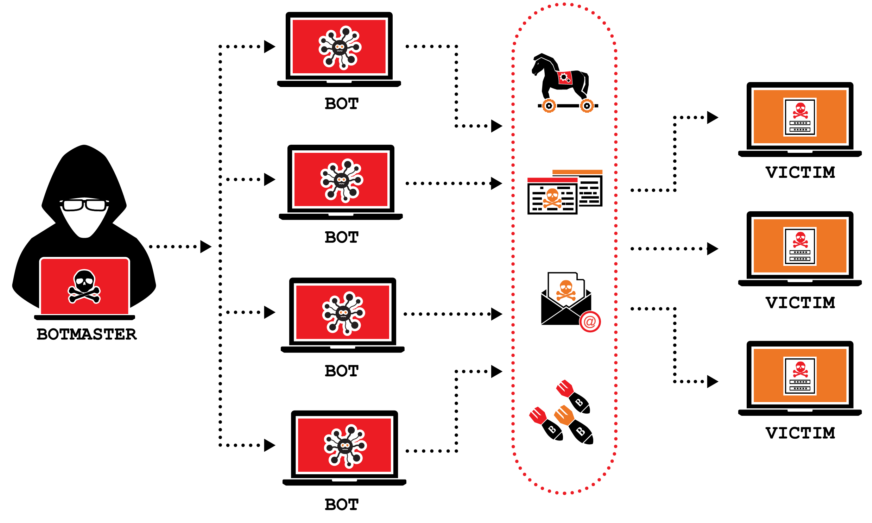
\includegraphics[width=0.95\linewidth]{pics/ddos2.png}
	\caption{DDoS攻击示意图}
	\label{fig:1}
\end{figure}

随着SDN技术的不断发展,越来越多的研究者开始探索基于SDN的DDoS攻击检测与防御方法。使用SDN技术进行流量控制和数据包分析,可以更加精细地分析DDoS攻击流量,准确地识别攻击源并进行切断,从而降低DDoS攻击的威胁。本文利用mininet平台模拟SDN架构进行网络流量监测研究,通过SDN架构实时监控流量信息的变化,深入挖掘网络流量中的潜在威胁,通过检测源地址和流量控制等方式,实现了高效的DDoS攻击检测和准确的攻击源定位。

%\end{multicols}
%
%\begin{figure}[H]
%	\centering
%	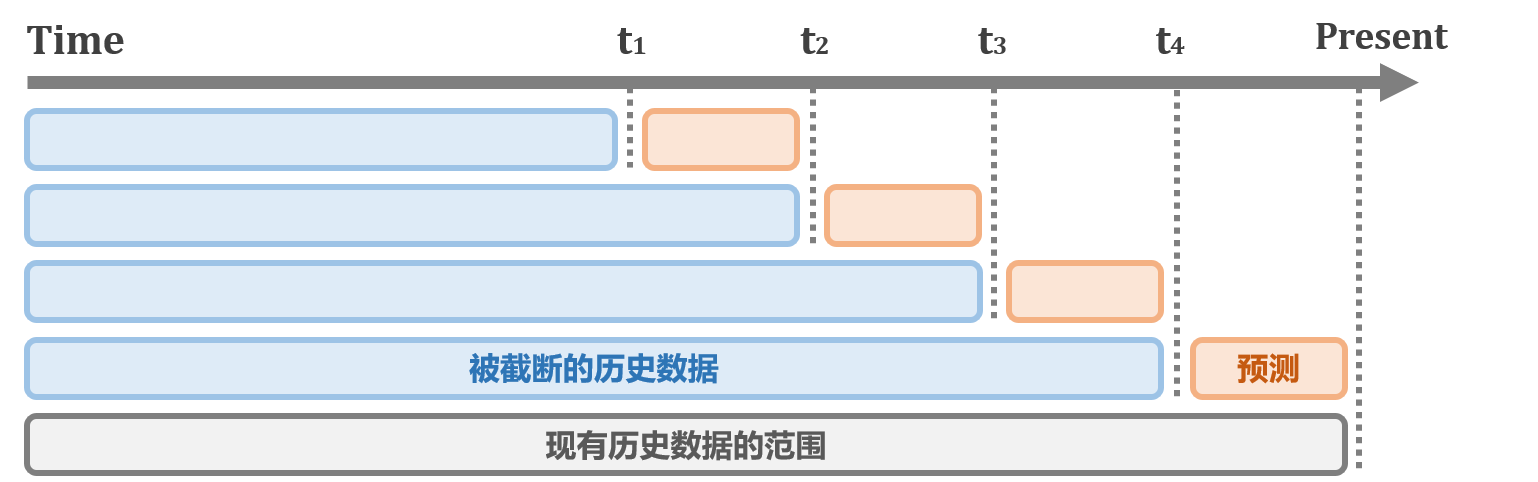
\includegraphics[width=14cm]{pics/bt1.png}\\
%	\caption{时间序列扩展窗口回测的概念示意图}\label{fig:backtest1}
%\end{figure}
%
%\begin{multicols}{2} 

%
%\begin{table}[H]
%	%\scriptsize
%	\footnotesize
%	\renewcommand{\arraystretch}{1.0}
%	\centering
%	\caption{\centering 模型的前移验证的预测评价指标统计对比}\label{tb:8}
%	\begin{tabular}{cccc}
%		\toprule[1.5pt]
%		&ARIMA&指数平滑&Prophet\\
%		\midrule[1pt]
%		 RMSE的中位数& 0.5440 &0.4785&\textbf{0.4055}\\
%		 RMSE的平均数& 0.5169&0.4529& \textbf{0.4126} \\
%		 MAE的中位数&0.4530 & 0.3435&\textbf{0.3045}\\
%		 MAE的平均值&0.4411 &\textbf{0.4115}&0.4116\\
%		 MAPE的中位数&108.84&92.38&\textbf{73.21}\\
%		 MAPE的平均值&134.32&119.56&\textbf{85.55}\\
%		\bottomrule[1.5pt]
%	\end{tabular}
%\end{table}
\section{相关介绍}
\subsection{DDoS攻击}
分布式拒绝服务攻击(DDoS),是一种通过网络对系统或服务进行攻击的方式,致使系统或服务无法正常提供服务,或导致系统瘫痪。DDoS攻击是一种袭击目标系统或服务的方式,它会占用网络带宽、系统资源和网络设备。本文中模拟使用的是Ping Flood DDoS攻击,这是一种最常见的DDoS攻击方式之一,它利用ICMP请求(Ping)向受害者发送大量伪造的网络数据,从而阻止受害者服务器的响应和服务,该攻击方式通常需要大量的机器共同协作实施,因此被称为分布式Ping Flood攻击。

Ping Flood DDoS攻击利用ping命令实现,它在网络上广泛使用以检测计算机和网络的通信。Ping Flood攻击向目标服务器发送大量的ping请求,并且在服务器响应时发送更多的请求。随着请求的不断增加,服务器最终无法正常响应请求,无法为合法用户提供服务,并可能导致网络设备和带宽资源被瓶颈。Ping Flood DDoS攻击通常采用分布式的方式进行,攻击者可以通过控制大量系统和设备,并通过Botnet等方式将请求分散到多个主机上,从而增加攻击的规模和强度。
\subsection{SDN架构}
SDN(Software Defined Network,软件定义网络)是一种新兴的网络架构,基于该架构,网络控制平面(control plane)和数据转发平面(data plane)被物理上分离开来。SDN中的网络设备只负责数据转发,并通过OpenFlow协议将数据转发行为反馈给SDN控制器。SDN架构的核心思想是将网络中的路由器、交换机等设备的数据转发和控制功能分离开来,将网络控制平面集中到一个名为SDN控制器的中心化控制器中。SDN控制器可以通过控制平面接口(如OpenFlow)管理网络中所有硬件设备,根据SDN网络的模型和策略实现数据包的转发和流量控制。

在SDN架构下,网络管理人员可以通过SDN控制器的相关工具和API来对网络进行管理和监控,包括网络拓扑、设备配置、访问控制、流量工程等。SDN技术可以对网络进行灵活的流量控制和优化,例如实现网络流量的负载均衡,统计网络流量和设备性能指标,优化路由路径等。SDN架构的优势主要体现在以下几个方面:
\begin{itemize}
	\item 简化管理:SDN架构通过集中式控制和管理,简化了网络管理的复杂性,减少了大量的手动配置和管理工作。
	
	\item 更灵活的流量控制:SDN架构中的SDN控制器可以动态地管理网络设备的数据转发,可以快速应对网络的变化,例如改变流量的路由路径,对网络拓扑进行调整等,从而避免网络的拥堵和流量泛滥。
	
	\item 更好的安全性:SDN架构的中心化控制器可以对网络设备进行统一的访问控制和审计,通过流量控制和权限管理等手段防止网络中的攻击和威胁。
\end{itemize}

\begin{figure}[H]
	\centering
	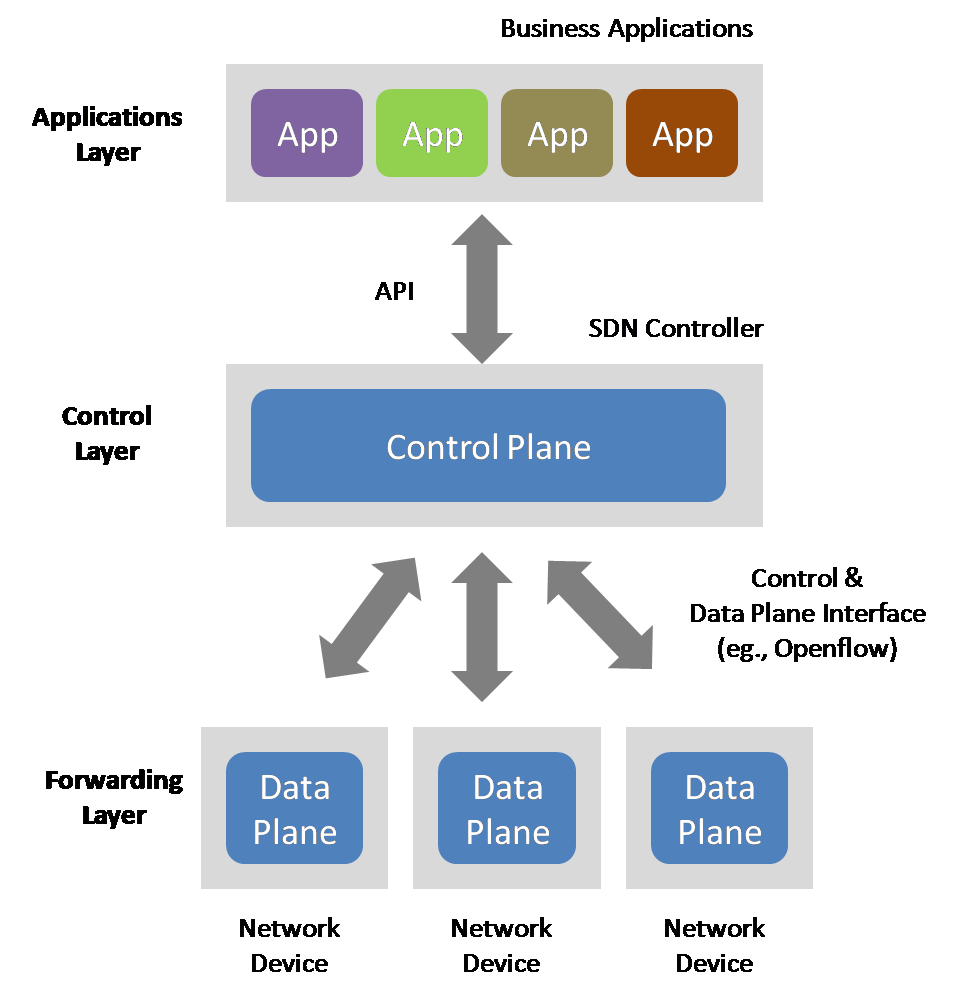
\includegraphics[width=0.95\linewidth]{pics/SDN.png}
	\caption{SDN架构示意图}
	\label{fig:1}
\end{figure}

总的来说,SDN架构是一种全新的、灵活的网络控制方式,为网络管理和安全提供了更加高效的方式。

\section{基于SDN的DDoS攻防模拟实验}
\subsection{实验环境}
为了便利模拟真实环境中的网络操作与架构,本次实验基于Ubuntu操作系统下的mininet网络仿真SDN平台。同时我们采用ryu控制器作为SDN控制器;利用postman进行API调试,对流表进行相关操作;利用适用于高速交换网络中的监控软件sFlow实时监控在DDoS攻击下流量信息的实时变化。具体环境如下:
\begin{itemize}
	\item CPU: 12th Gen Intel(R) Core(TM) i9-12900K
	\item OS: Ubuntu 18.04 LTS
	\item Tools: floodlight 1.2, mininet 2.3.0, Sflow-RT 3.0
	\item Java 1.8.0, Apache Ant 1.10.13
\end{itemize}
\subsection{实验模拟过程}
首先基于mininet仿真SDN平台搭建网络拓扑,如下图所示:
\begin{lstlisting}
sudo mn --controller=remote, ip=127.0.0.1, port=6653 --topo=single, 3
\end{lstlisting}
% TODO: \usepackage{graphicx} required
\begin{figure}[H]
	\centering
	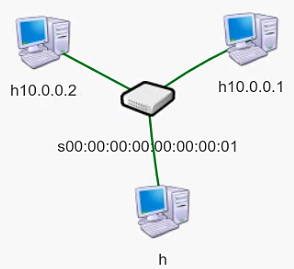
\includegraphics[width=0.55\linewidth]{pics/screenshot001}
	\caption{拓扑结构网络搭建}
	\label{fig:screenshot001}
\end{figure}
\subsubsection{DDoS攻击模拟}
首先在虚拟交换机配置sFlow Agent,以便sFlow Collector获取流量信息进行分析和呈现。
\begin{lstlisting}
sudo ovs-vsctl -- --id=@sflow create sflow agent=eth0 target=\"127.0.0.1:6343\" sampling=10 polling=20 -- -- set bridge s1 sflow=@sflow
\end{lstlisting}
\end{multicols}
\begin{figure}[H]
	\centering
	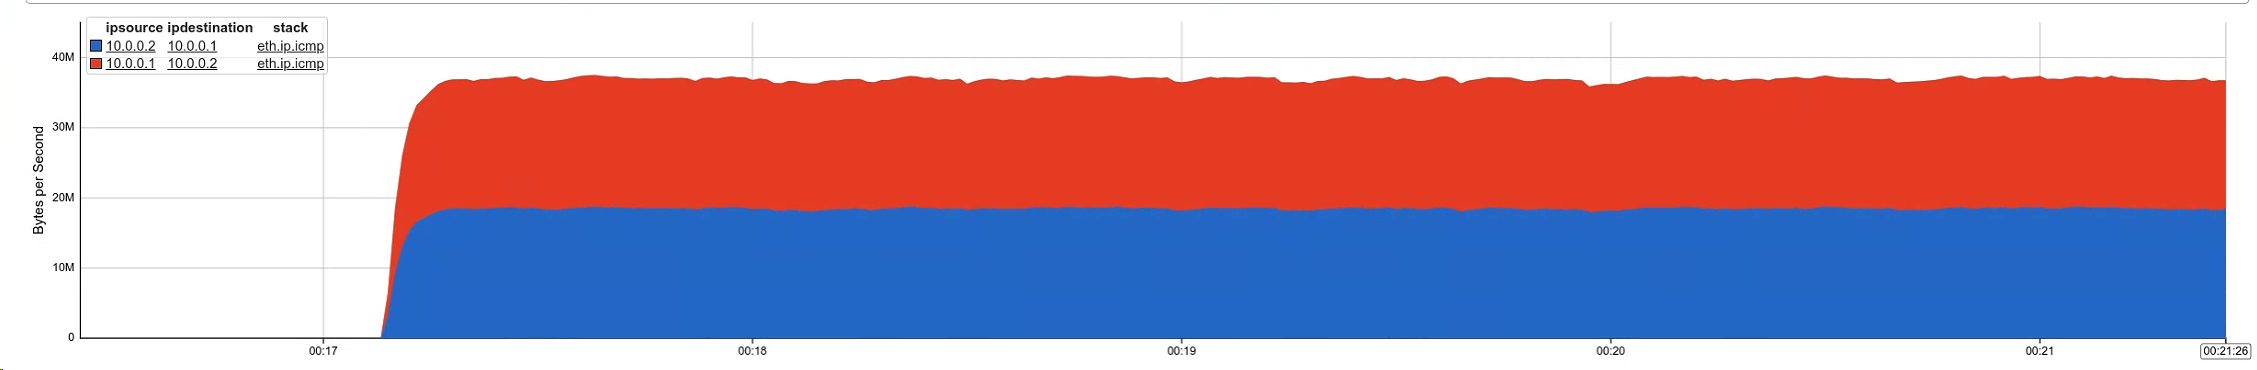
\includegraphics[width=0.9\linewidth]{pics/screenshot017}
	\caption{DDoS攻击期间交换机流量}
	\label{fig:screenshot017}
\end{figure}

\begin{figure}[H]
	\centering
	\subfigure[DDoS攻击前流量监测]{
		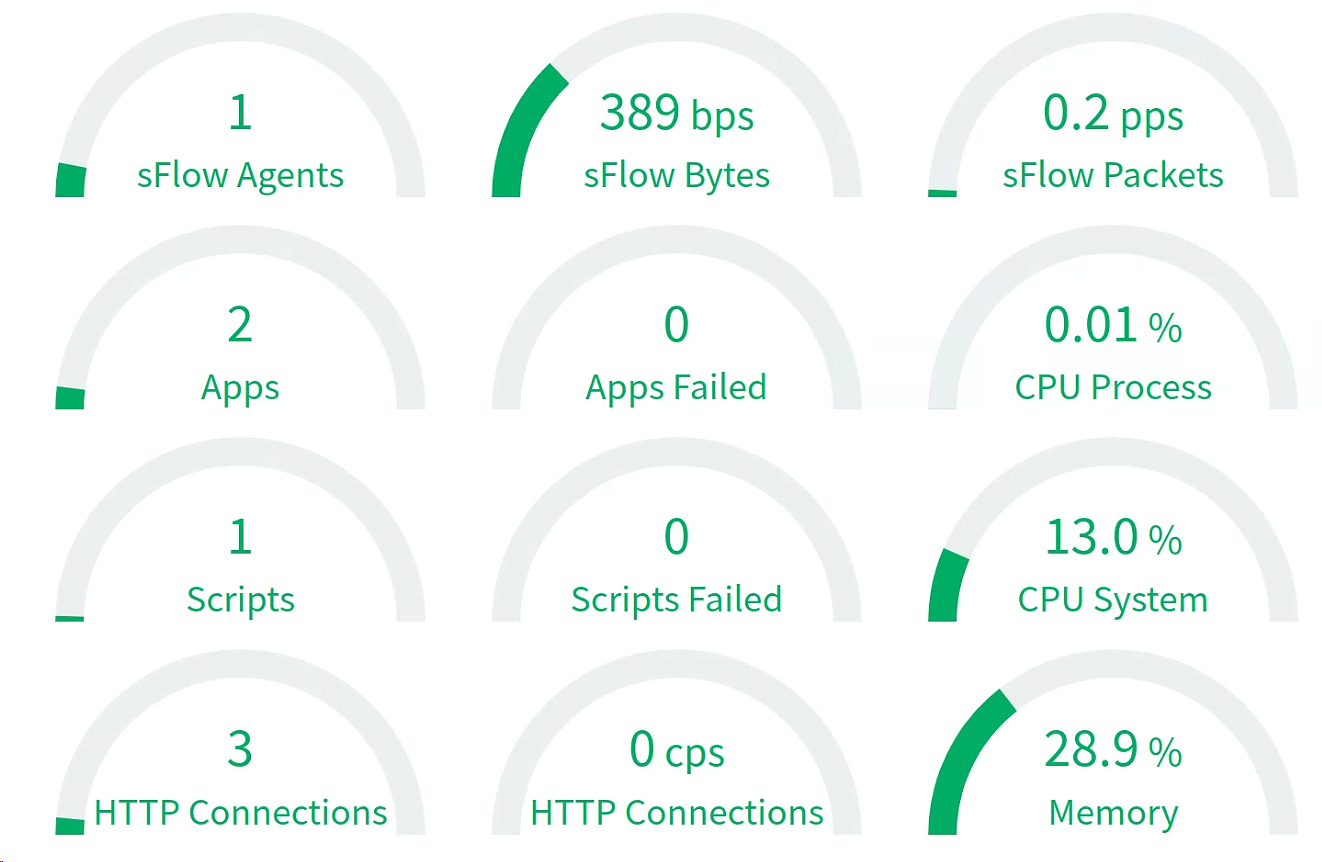
\includegraphics[width=0.45\linewidth]{pics/screenshot016.png}
		%\caption{fig1}
	}
	\quad
	\subfigure[DDoS攻击期间流量监测]{
		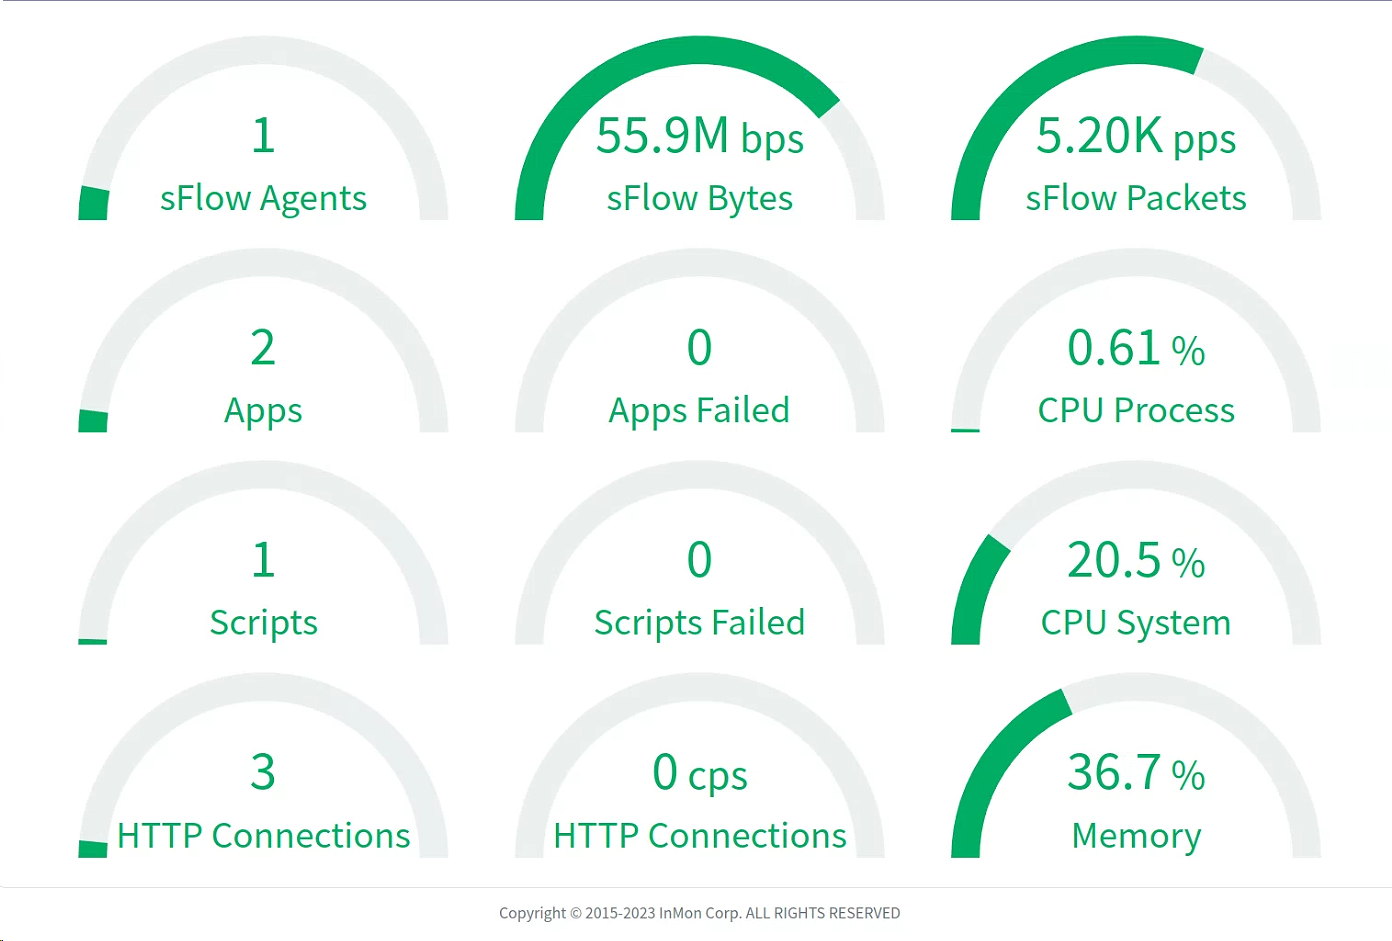
\includegraphics[width=0.45\linewidth]{pics/screenshot015.png}
	}
\end{figure}
\begin{multicols}{2}
	
然后切换到mininet控制台窗口,打开Host1和Host2的终端,并在Host1上启动一个 http 服务:
\begin{lstlisting}
mininet> xterm h1 h2
python -m SimpleHTTPServer 80&
\end{lstlisting}
接下来进行DDoS模拟攻击,在 mininet终端中执行
\begin{lstlisting}
h2 ping -f h1
\end{lstlisting}
即模拟h2对h1的Ping Flood DDoS攻击。攻击期间流量监测见图4与图5。可以看出当,命令执行后,监测的传输流量剧增,CPU占用和内存占用也大幅度增加。
\subsubsection{DDoS 攻击防御}
在监测到流量异常之后,需要利用RYU控制器向OpenFlow交换机下发流表,抑制攻击流量。流表是交换机进行转发策略控制的核心数据结构。交换机芯片通过查找流表项来决策进入交换机网络的数据包执行适当的处理动作。下发一条流表则好比一条指令,告诉交换机收到数据包之后该做什么。由于先前的DDoS采用的Ping Flood攻击,因此我们需要下发流表,将攻击流抵消掉。在静态流表下发之后,可以发现流量迅速下降,h2向h1泛洪的数据包被迅速地完全Drop。
\end{multicols}

\begin{figure}[H]
	\centering
	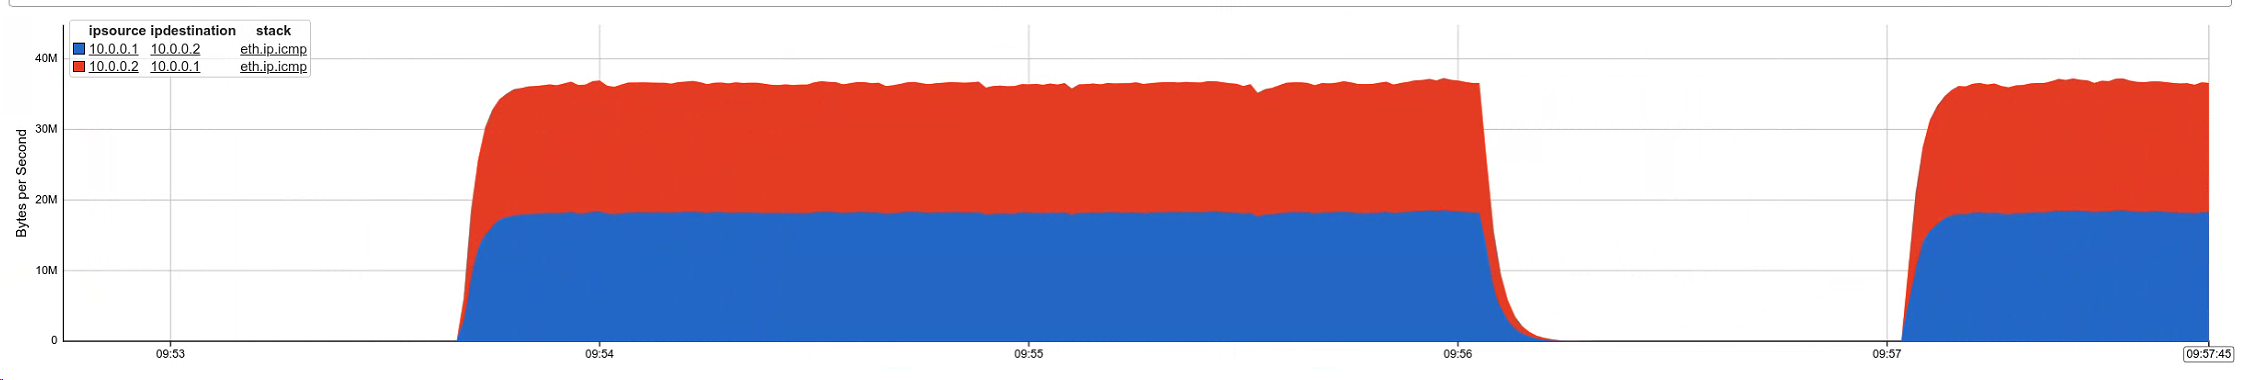
\includegraphics[width=0.9\linewidth]{pics/screenshot00122}
	\caption{下发流表后的流量监控}
	\label{fig:screenshot00122}
\end{figure}

\begin{multicols}{2}
\section{总结}
本文基于mininet平台模拟仿真SDN架构研究DDoS的攻击和防御,为真实网络监控提供一定的借鉴意义。利用sFlow 来实时监控传输流量信息的变化,并实时显示网络流量以得到更加直观的结果。对于传统网络的部署,是无法做到像SDN那样可以实时监控端口传输流量信息的。利用SDN架构的网络拓扑结构,以中央控制的方式部署网络结构相较于传统的网络部署方式更加具有防御性,对抑制DDoS攻击更加有效。通过SDN技术,我们可以对网络流量进行实时监控与提取分析,并能够及时的对流量进行调整比如QoS,负载均衡,DDoS流量过滤等,具有丰富的实践意义。
\end{multicols}




















